\documentclass[journal]{IEEEtran}
%\usepackage{ctex}
\bibliographystyle{unsrt}

\usepackage{graphicx}
\usepackage{float}
\graphicspath{{figures/}}


\ifCLASSINFOpdf
\else

\fi


% IEEEtran contains the IEEEeqnarray family of commands that can be used to
% IEEEtran.cls'  captionsoff option. Some IEEE journals/societies require that
% IEEE papers do not typically make use of \caption[]'s optional argument,

%显示直立文本: \textup{文本}
%意大利斜体: \textit{文本}
%slanted斜体: \textsl{文本}
%显示小体大写文本:  \textsc{文本}
%中等权重: \textmd{文本}
%加粗命令: \textbf{文本}
%默认值: \textnormal{文本}

\hyphenation{op-tical net-works semi-conduc-tor}


\begin{document}



\title{Bare Demo of IEEEtran.cls\\ for IEEE Journals}

\author{Michael~Shell,~\IEEEmembership{Member,~IEEE,}
        John~Doe,~\IEEEmembership{Fellow,~OSA,}
        and~Jane~Doe,~\IEEEmembership{Life~Fellow,~IEEE}% <-this % stops a space
\thanks{ some information is here 
	M. Shell was with the Department
of Electrical and Computer Engineering, Georgia Institute of Technology, Atlanta,
GA, 30332 USA e-mail: (see http://www.michaelshell.org/contact.html).}% <-this % stops a space
\thanks{J. Doe and J. Doe are with Anonymous University.}% <-this % stops a space
\thanks{Manuscript received April 19, 2005; revised August 26, 2015.}}


\maketitle

% As a general rule, do not put math, special symbols or citations
% in the abstract or keywords.
\begin{abstract}
We present a real-time indoor relocation system based only on 2D-laser sensor. Our system processed 2D laser data into multi-channel image and occupancy grid map, which were used as the input of a Convolutional Neural Network(CNN). Our system trains a convolutional neural network to regress the 3-DOF robot pose from a channel-superposition image by  multi-channel images and occupancy grid maps with no need of additional optimisation. Our algorithm can obtain approximately 2m and $5^{\circ}$ accuracy indoors, in which our system distributes particles depend on particle filter algorithm. Our system only uses five layers convolution and four layers fully connected network structure, which can achieve the effect of rapid training.
\end{abstract}

% Note that keywords are not normally used for peerreview papers.
\begin{IEEEkeywords}
Relocation, 2D-laser data,  Multi-channel image, Occupancy grid map
\end{IEEEkeywords}


\IEEEpeerreviewmaketitle

\section{Introduction}
\IEEEPARstart{O}ver the past few decades, Indoor robotics have made an amazing improvement. Indoor robots rely on lasers alone  have been able to navigate smoothly \cite{lingemann2005high}, \cite{csorba1997simultaneous}. In traditional method, particle filter algorithm is used in the task of location and navigation indoors \cite{fox1999monte}, \cite{aghili2016robust}. However the problem of robot lost or kidnapped is to hard for traditional method to solve. One of the main techniques to solve those kind of problem is to let robot know it's pose approximately only depends on the sensor when the robot is started for the first time. 

In recent years, there are more and more approaches aiming at robot relocation indoors. In \cite{williams2007real}, an idea of  extending recent advances in key point recognition was presented, however, this is no information when robot start for the first time. A hypotheses was proposed in \cite{williams2007real}, which found with relocation procedure can be used to initialize a generic localization algorithm before the robot starts moving, or when the robot gets lost. However, traditional methods can not solve the problem of robot relocation in an excessively similar environment. Popular past works have considered posture regression. In \cite{kendall2015posenet}, a network structure based on Googlenet \cite{szegedy2015going} is used to  regress a 6-DOF pose.The image obtained based on depth camera contains more feature points, however, this method can not be used under the condition of insufficient illumination, and it consumes a lot of computation when training the network structure based on Googlenet. Similar ideas are also introduced in \cite{kuse2019learning}, which is able to recover from complicated kidnap scenarios and failures online in real-time. 

\begin{figure}
	\centering
    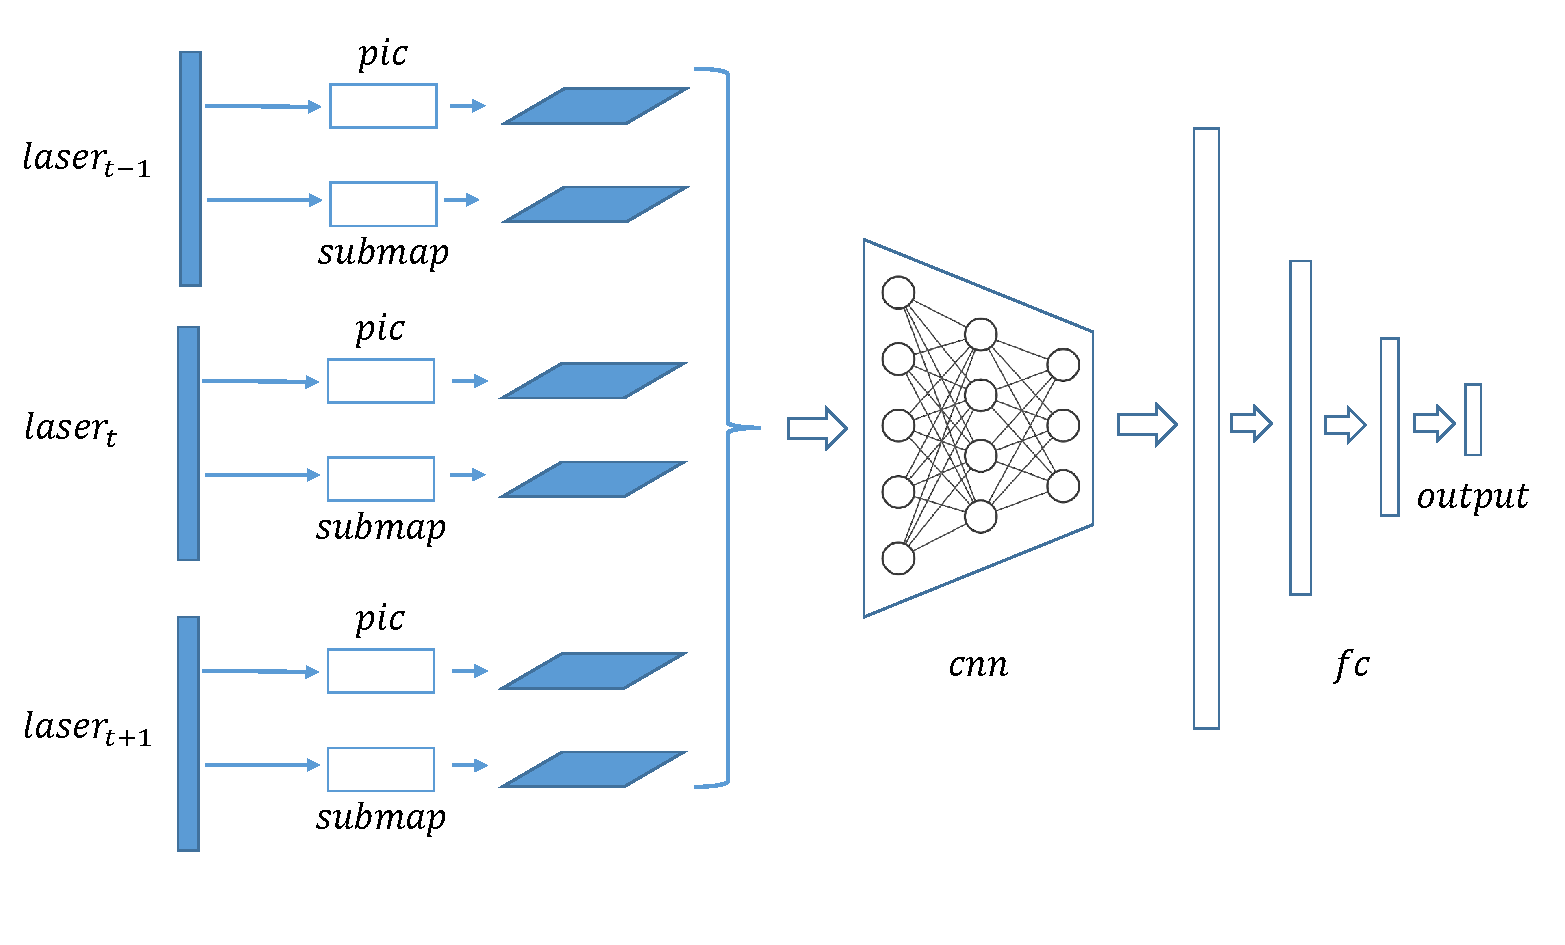
\includegraphics[width=0.45\textwidth]{figure1.pdf}
    \caption{ System overview of the proposed relocation algorithm for robot relocalization indoors. The laser data is processed into RGB image and occupancy grid map. The image and map  were superpose into 6-channel image,while 3 6-channel images,which represent laser data t-1,t,t+1respectively, were superpose into a 12-channel image.The 12-channel image is used as the input of a  convolutional neural network(CNN),while the output is a 3-DOF  posture including pose and orientation.	}
    \label{fig:frame}
\end{figure}

In order to solve the kidnapped robot problem when robot restart from any point in the similar indoor environment, we  introduce a novel relocation  algorithm in this paper. Our proposed system, Relocation-Net, takes a multi-channel image and regresses the robot's 3-DOF pose relative to a scene. Fig.\ref{fig:frame} demonstrates the system structure. The algorithm is simple in the fact that it consists of a convolutional neural network(CNN) trained to regress the robot's orientation and position. 

The paper's main contribution are the 2D-laser data processing method and the deep convolutional neural network robot pose regressor. We introduced a novel technique to process the 2D-laser data, which makes it possible for indoor robot to regress pose relying only on 2D-laser sensor. Our main contributions are as follows:

\begin{itemize}
	\item  A novel method to process 2D-laser data in order to  increase the features of the input of CNN, which is so hard that it is impossible to regress only depend on 2D-laser data.
	
	\item A new method to regress robot 's pose indoor. To the best of our knowledge, this is the first algorithm to regress robot’s 3-DoF pose depends on the 2D-laser merely.
\end{itemize}

The proposed deep learning based  robot's pose regression system can relocate the robot approximately 2m far away from the real pose of robot when robots start for the fist time indoors, while particle filter algorithm is able to operate without the kidnapped robot problem because the area to distribute particles  is constrained to within 2m from the true pose.

The rest of this paper is organized as follows. Section II reviews related work. Following a system overview in Section III, Section IV presents the proposed 2D-laser data process method.  . In Section V, the CNN based robot pose regression method  is introduced to refine poses predicted from the network. Experimental results are given in Section VI. The conclusions are drawn in Section VII.

%\hfill mds
 
%\hfill August 26, 2015

\section{relate works}

Robot relocation aims for let robot know where it is. Classical methods tend to use the information of surrounding environment observed by sensors. In this paper, we focus on using 2D-laser data merely to regress robot  3-DOF  posture including pose and orientation.

\subsection{Robots Relocation Indoors}

In resent years, researchers have made a lot of effort to try to optimize the performance of robot relocation indoors. Serval sensors were  taken into consideration. Sonar data is used in \cite{lim2000mobile}, which presented a method for relocation of a mobile robot indoors using sonar data. In this paper a physically-based sonar sensor model was used to characterize the geometric constraints provided by echolocation measurements of different types of objects. Individual range returns were used as data features in a constraint-based search to determine the robot's position. However,the sonar detection range is directly limited by the band loss (high-frequency radar must be used to detect the distance), and pedestrians are not perceived, and it is impossible to accurately simulate all surrounding obstacles.
Paper \cite{yang2019rapid} proposed an offline map construction algorithm based on map elements and key frame database which designed a mobile robot fast positioning method. Similar ideas are also introduced in     \cite{castellanos1997building}, this paper explored the correlation between geometric entities from the perspective of map composition, and showed that maintaining the correlation and hypothesis independence between map entities can reduce these uncertainties which can obtain more accurate estimation in robot relocation.  Robot relocation based ORB-SLAM2 \cite{mur2015orb} is used and improved in \cite{mur2017orb}, \cite{engel2014lsd}, \cite{yang2016pop}, \cite{mur2017visual}. Robot  relocation based on orb-slam algorithm can extract more observation features and has better robustness. However, such algorithms not only consume a lot of computing resources, but also have very strict requirements on lighting conditions.

2D-laser based robot indoors location technique was presented in \cite{thrun2005probabilistic}, considerable techniques are introduced with respect to the state of the robot indoors, which including Kalman Filter \cite{kalman1960new}, Extended Kalman Filter \cite{bailey2006consistency}, Unscented Kalman Filter \cite{martinez2005unscented}. Moreover, paper \cite{sim2006design} proposed a particle filter-based monocular SLAM algorithm which could  avoid linearization appear in   \cite{thrun2005probabilistic}, \cite{kalman1960new}, \cite{bailey2006consistency}, \cite{martinez2005unscented}. The particle filter algorithm implements recursive Bayesian filtering by a non-parametric Monte Carlo \cite{robert2013monte} simulation method, which estimates the indoor robot's pose go through initializing the particle, calculating each particle's weight, and particle resampling. Particle filtering algorithm is a traditional algorithm with strong robustness, but the robot kidnapped  in similar environment is fatal.


\subsection{Deep Learning based Robots Relocation Indoors }

Most of existing deep learning based robot relocation methods are vision based  \cite{kendall2015posenet}, \cite{kuse2019learning}, \cite{zhou2017unsupervised}. Other machine learning techniques are employed for the loop-closure problem \cite{yin2018synchronous}  \cite{chen2017deep}. Paper \cite{li2017deep} proposed a 2d scan matching method based on deep learning, in which using the Hector SLAM \cite{kohlbrecher2011flexible} to achieve a good result. However, the benefits of deep learning for relocation depends on 2D-laser merely have not been fully explored.

\section{system overview}

In this section, an CNN based robot indoors pose estimation system is briefly described. Fig. \ref{fig:frame}  shows the proposed system framework. It consists of two parts: a 2D-laser data processor and a CNN based robot pose estimation.

The CNN based pose estimation system is composed of a laser data processor with a CNN based point cloud feature extraction. The laser processor is designed to process 2D-laser data into images and occupancy grid maps, which is a novel technique to add features of the input of CNN. A CNN is designed to extract features from multi-channel images processed form laser data. Meanwhile, particle filter algorithm is not abandoned in this paper, which is used to distribute particles within a certain range around the position predicted by our system.

\section{CNN based relocation system}

This section presents the proposed CNN based system for robot  indoors relocation in detail. The cost functions designed for training the CNN are also described.


\subsection{2D-laser Processor}

\begin{figure}
	\centering
	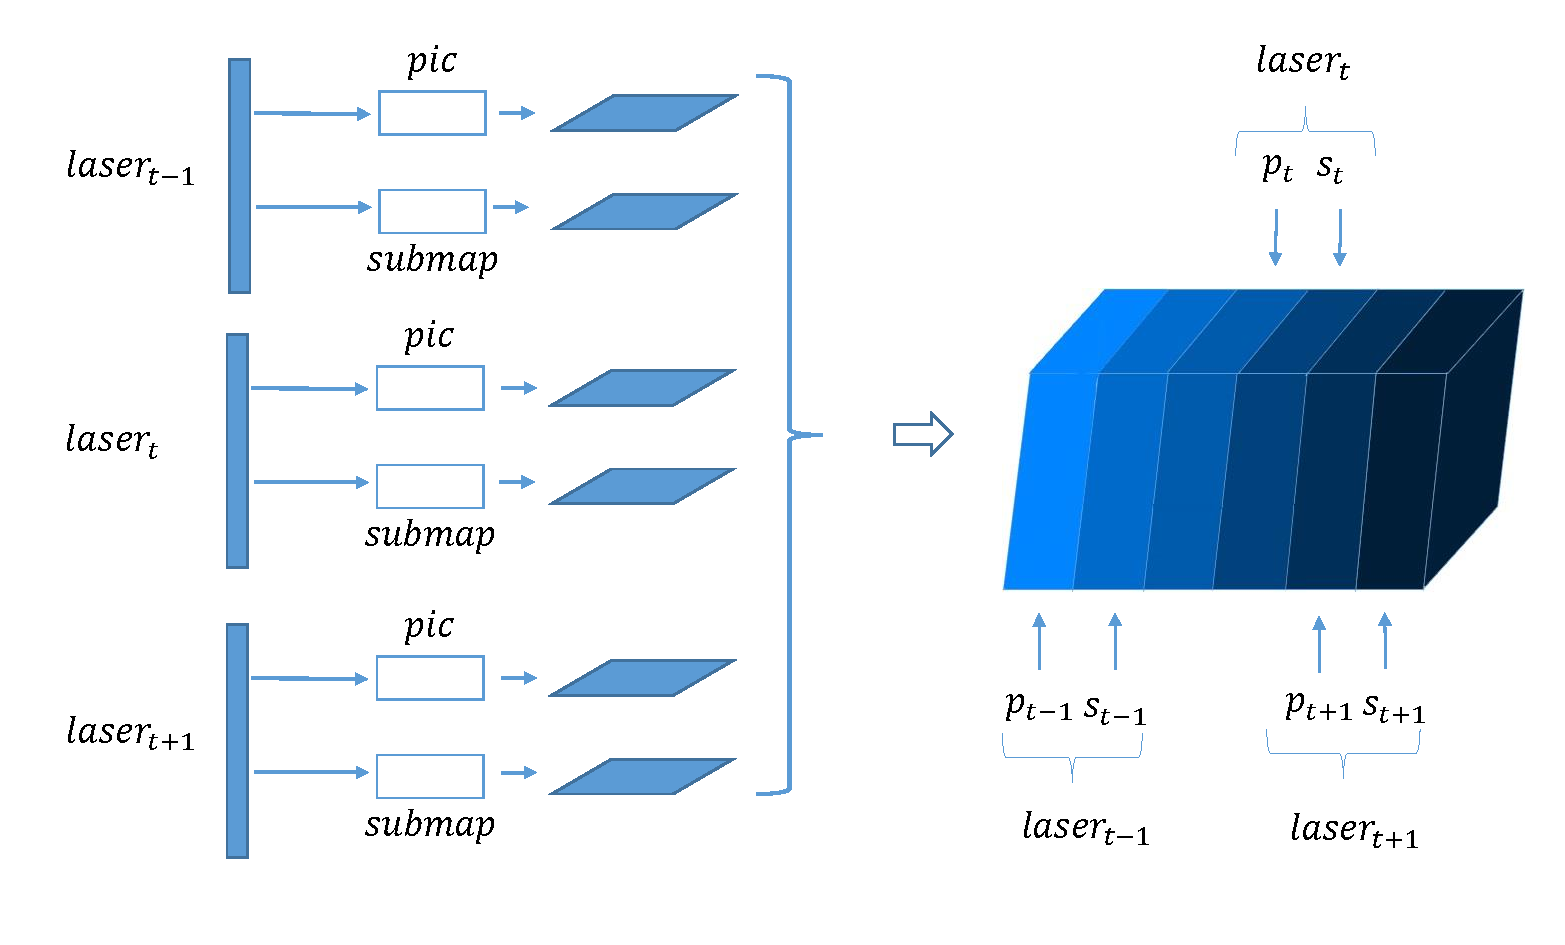
\includegraphics[width=0.45\textwidth]{figure3.pdf}
	\caption{ System overview of 2D-laser processor We process three frames of continuous laser datas,every single-frame 2D-laser data  was processed into a RGB image and an occupancy grid map.The image and map  were superpose into 6-channel image,while 3 6-channel images,which represent laser data $t-1$,$t$,$t+1$respectively, were superpose into a 18-channel image.The 18-channel image is used as the input of a  convolutional neural network(CNN).}
\end{figure}


\begin{figure*}[htb]
	\centering
	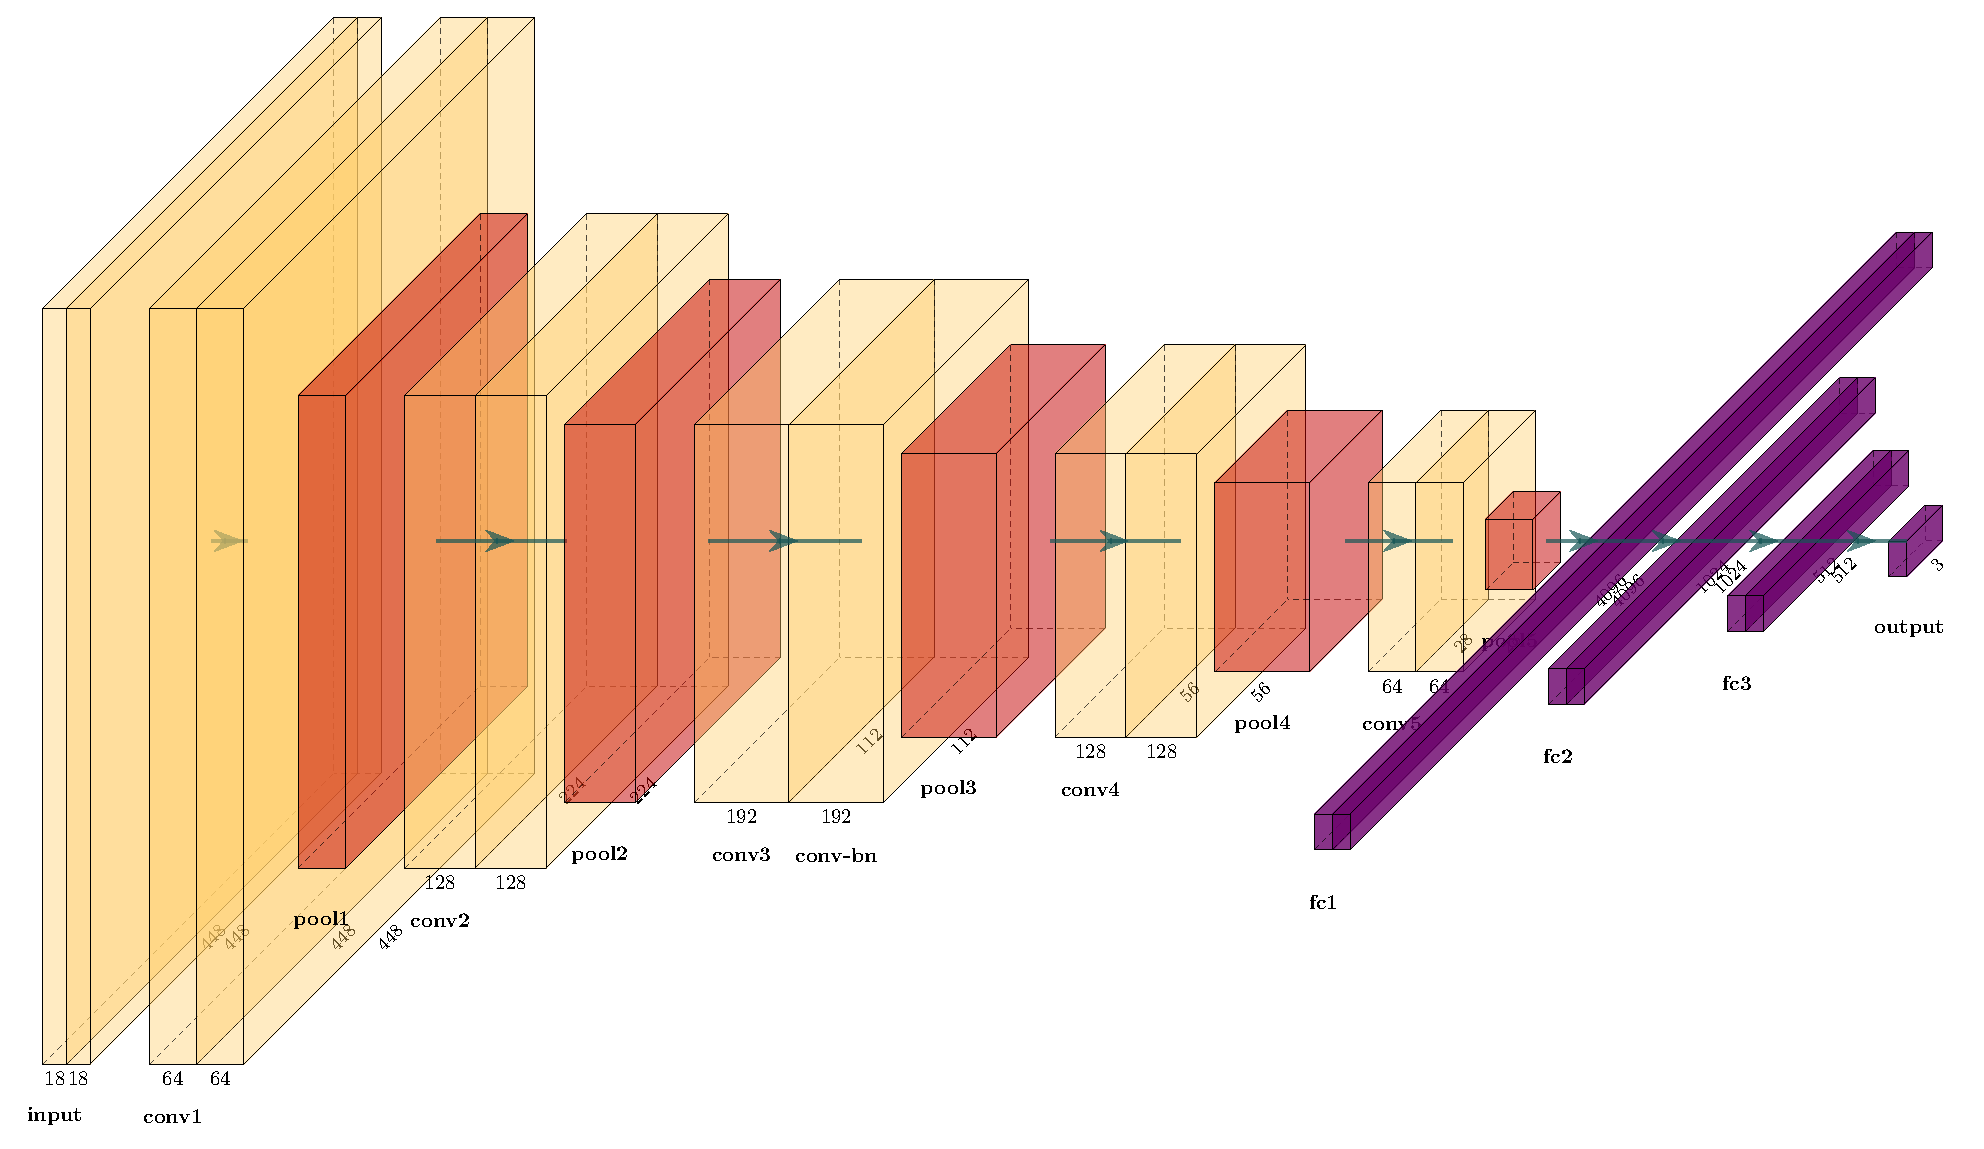
\includegraphics[width=0.8\textwidth]{cnn_bn.pdf}
	\caption{ Architecture of the CNN network in proposed data fusion system. The network consists of five 2D convolutional layers  with three fully connected layers.The output of the network is the 3-DOF  posture including pose and orientation } 
	 \label{fig:curl1}
\end{figure*}


2D-laser laser is used as observation data in particle filter algorithm. Its robustness and characteristics that are not affected by the light source are its advantages as observation data in traditional algorithm. Howerer, single-frame 2D-laser data has fewer features, making it impossible to accurately regress the robot pose as an input of the deep network \cite{li2017deep}. We presented a novel way to process 2D-laser data to  increase its features significantly.


\subsection{CNN based Pose Regression}

In the reason that convolutional layers can be interpreted as transforming inputs into feature representation effectively, a neural network, in this paper, was designed  to  learn useful features representation of the  multi-channel  image automatically. The features extracted form multi-channel  image went through five convolutional layers and was pulled into 1 dimension.  The fully connected layers followed  map the learned distributed feature representation to the sample tag space. The output of the last fully connected layers is a $1*3$ vector including $1*2$ pose and $1*1$ orientation.

\begin{table}[h]
	\centering
	\caption{ Configuration of the CNN}
	\begin{tabular}{ccccc}
		\hline
		Layer & Kernel Size & Padding & stride & \begin{tabular}[c]{@{}c@{}}Nunber of \\ Channerls\end{tabular} \\ \hline
		conv1 & 7           & SAME    & 2      & 64                                                             \\
		conv2 & 5           & SAME    & 2      & 128                                                            \\
		conv3 & 5           & SAME    & 2      & 192                                                            \\
		conv4 & 3           & SAME    & 2      & 128                                                            \\
		conv5 & 3           & SAME    & 2      & 64                                                             \\ \hline
	\end{tabular}
	 \label{tabCNN}    
\end{table}

The configuration of the CNN is outlined in TABLE \ref{tabCNN}. The input of the network is a multi-channel  image processed form 2D-laser data. There are five convolutional layers along with five pooling layers, each of which has a rectified linear unit (leaky-ReLU \cite{xu2015empirical}) activation.  Following the last convolutional layer, four fully connected layers are used to extract a global feature and regress the pose we need.


\subsection{Cost Function }

The cost function is designed to train the CNN so that its predicted poses are close to the ground truth. Specifically, the cost function contains two parts: a  pose error with an angle error.

\begin{figure}[h]
	\centering
	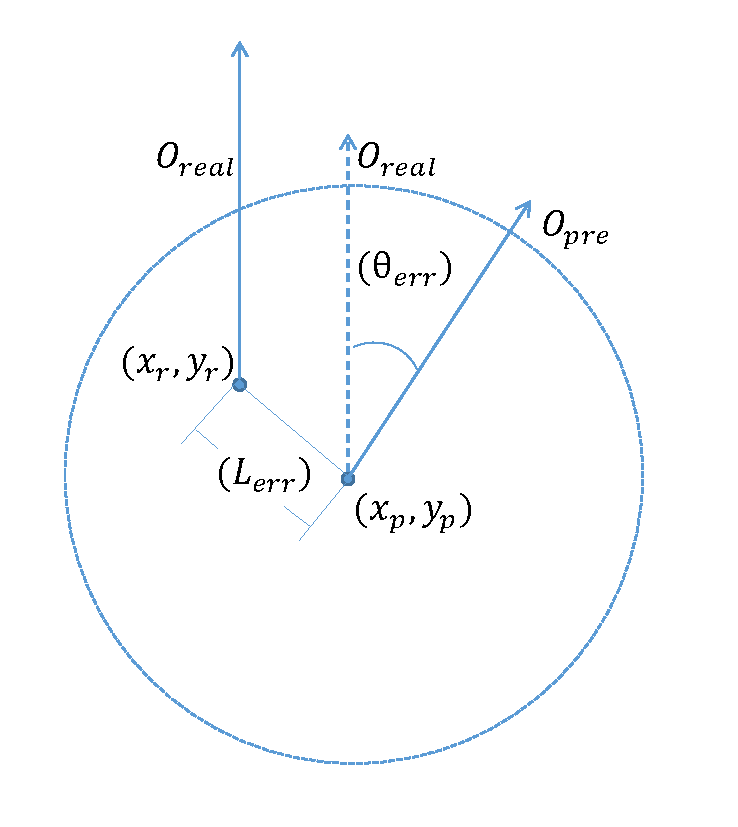
\includegraphics[width=0.4\textwidth]{cost.pdf}
	\caption{ Illustration of the way to calculate the errors between the predicted location and the ground truth.  }
	 \label{fig:cost}
\end{figure}

\subsubsection{Pose error }
 Pose error is formulated as the euclidean distance between the predicted positions the ground truths. The function aims to minimize the euclidean distance between the ground truth poses and the estimated ones from the network. The error function is as follows:
 \begin{equation}
 	L_{err}= \frac{1}{n}\sum_{i=1}^{n}\{||\hat{x}-x||^2_2+||\hat{y}-y||^2_2\}
 \end{equation}

where $|| \cdot ||^2_2 $ is the 2-norm,  and n is the batch size.


\subsubsection{Orientation error }
Two methods are considered to calculate the orientation error in this paper.
\paragraph{quaternions}
The first way is shown in Formula\ref{eq:loss1},we used the form of quaternion to calculate the error between the predicted value and the ground truth.

\begin{equation}
	 \Theta_{err}= \frac{1}{n}\sum_{i=1}^{n}\beta||\hat{q}-\frac{\hat{q}}{||q||_2}||   \label{eq:loss1}
\end{equation}

where $|| \cdot ||^2_2 $ is the 2-norm,  and n is the batch size,and q means the quaternion representing the orientation,and $\beta$  is a factor to balance the weight of positions and orientations.

Quaternions is a good choice to represent orientation, because arbitrary 4-D values are easily mapped to legitimate rotations by normalizing them to unit length.

\paragraph{angle}
The second way is shown in Formula\ref{eq:loss2},we used form of angle to calculate the error between the predicted value and the ground truth.

\begin{equation}
\Theta_{err}= \frac{1}{n}\sum_{i=1}^{n}\beta||\hat{\theta} -\theta ||^2_2 \label{eq:loss2}
\end{equation}

where $|| \cdot ||^2_2 $ is the 2-norm,  and n is the batch size,and $\theta$ means the angle representing the orientation,and $\beta$  is a factor to balance the weight of positions and orientations.

In this paper we describe the convolutional neural network (convnet) we train to estimate robot pose directly from a multi-channel image  image. Our network outputs a pose vector $V_o$, given by a 2D robot position x and orientation
represented by angle $\theta$:

\begin{equation}
	V_o=[x,\theta]  \label{eq:out}
\end{equation}

We chose angles as our orientation representation, because arbitrary 1D values are easily mapped to legitimate rotations in 2D space. This is a simpler process than the 4D values  normalization and orthonormalization required of rotation matrices.

\section{Experiment Results}
In this section, we evaluate the performance of the proposed system. The CNN model is trained by using data collected from a true environment, and tested on a real Pioneer 3-DX robot running in the same environments. As we know,the particle filter algorithm derives the pose of the indoor robot through four steps, which including particle initialization, particle motion update, particle observation update and calculate the posture in the end \cite{thrun2005probabilistic}. Here we use the posture calculated from the last step of the particle filter algorithm as the ground truth of CNN and use the single-frame laser data which is used to calculate the posture as the data to be preprocessed into multi-channel image.

\begin{figure}[H]
	\centering
	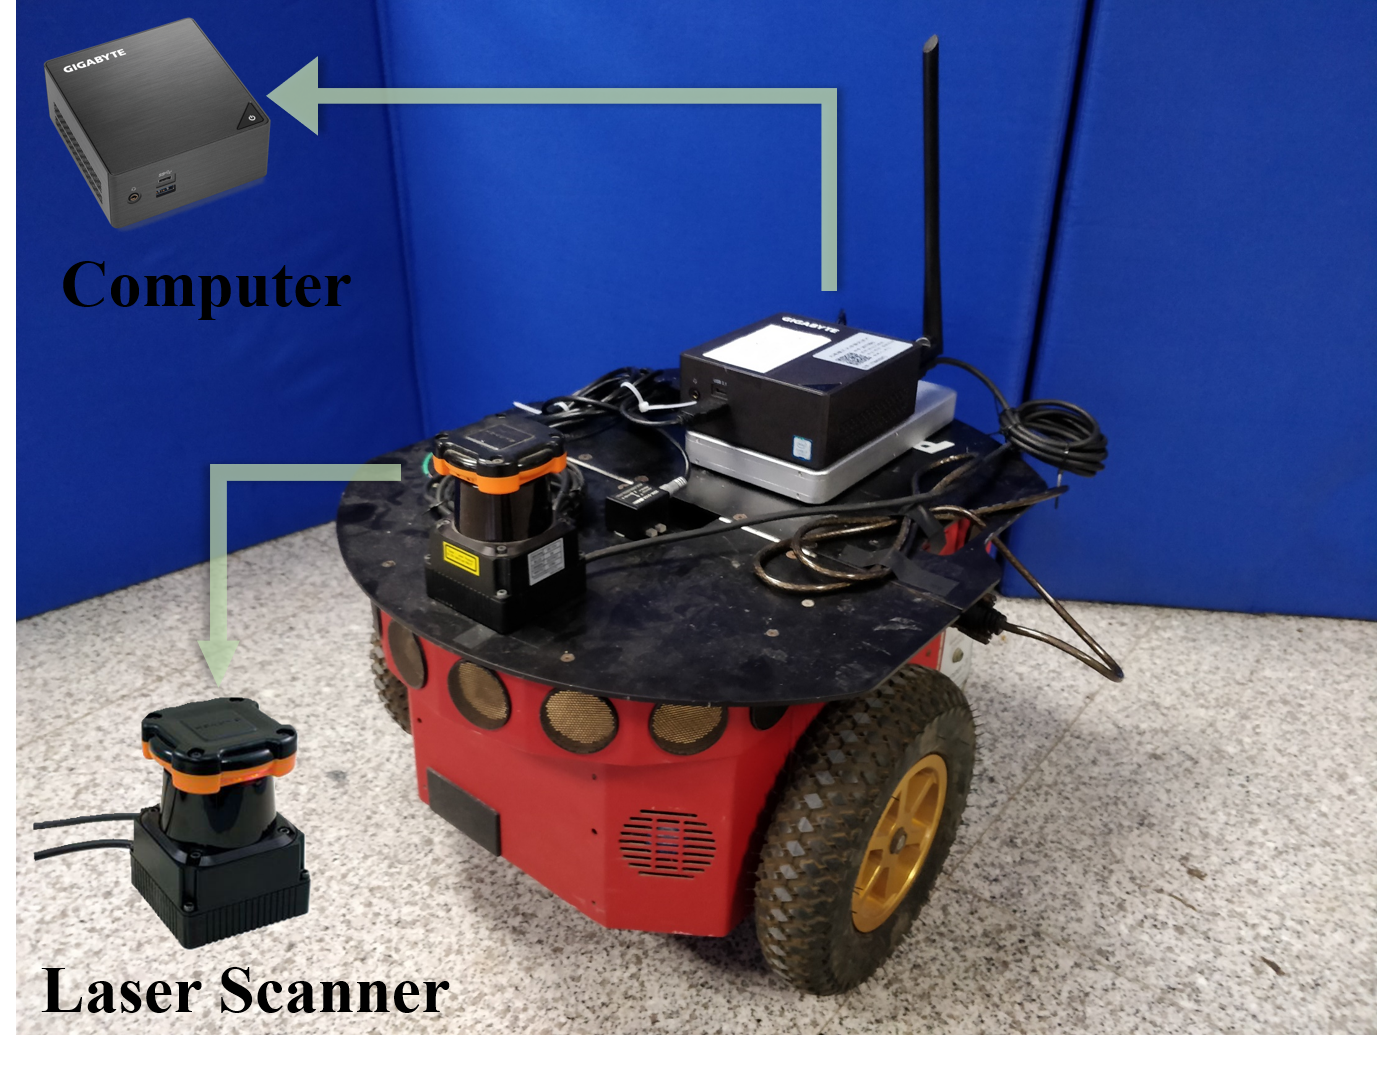
\includegraphics[width=0.4\textwidth]{robot.png}
	\caption{The setup of the mobile robot equipped with a Hokuyo laser scanner.} 
	\label{fig:robot}
\end{figure}

\begin{figure}[H]
	\centering
	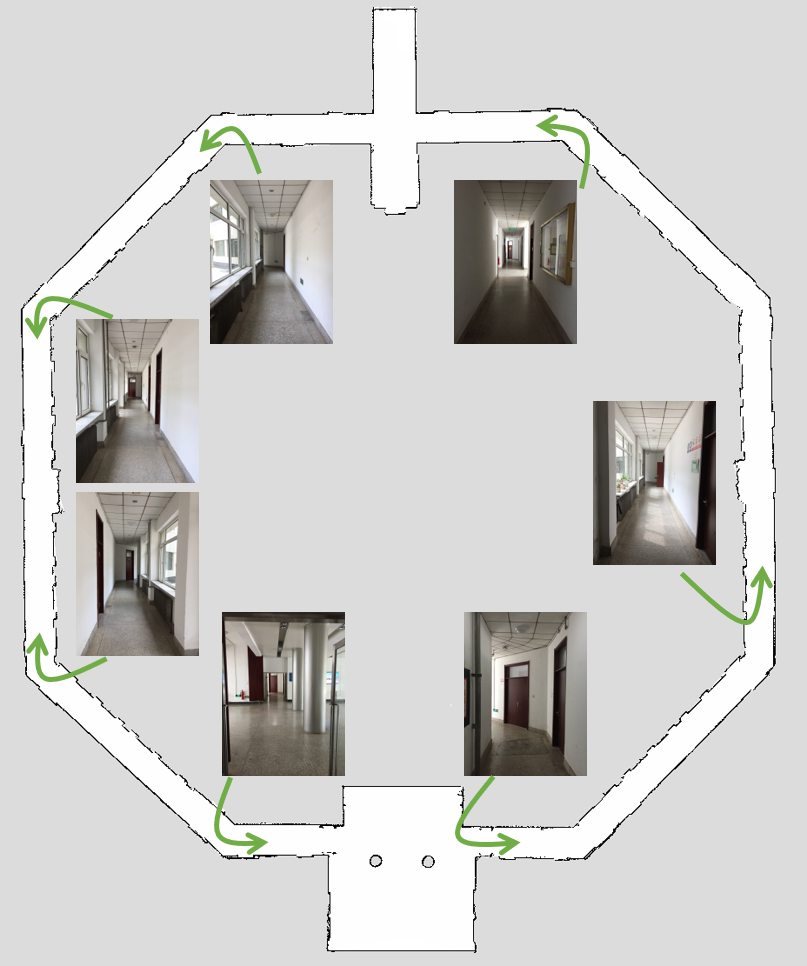
\includegraphics[width=0.4\textwidth]{map1.png}
	\caption{Priori map \uppercase\expandafter{\romannumeral1} of the real environment used to collect the data set.The white pixels represent the area without obstacles,the black pixels represent areas with obstacles and the gray pixels represent unknown area.} 
	\label{fig:map1}
\end{figure}

\begin{figure}[H]
	\centering
	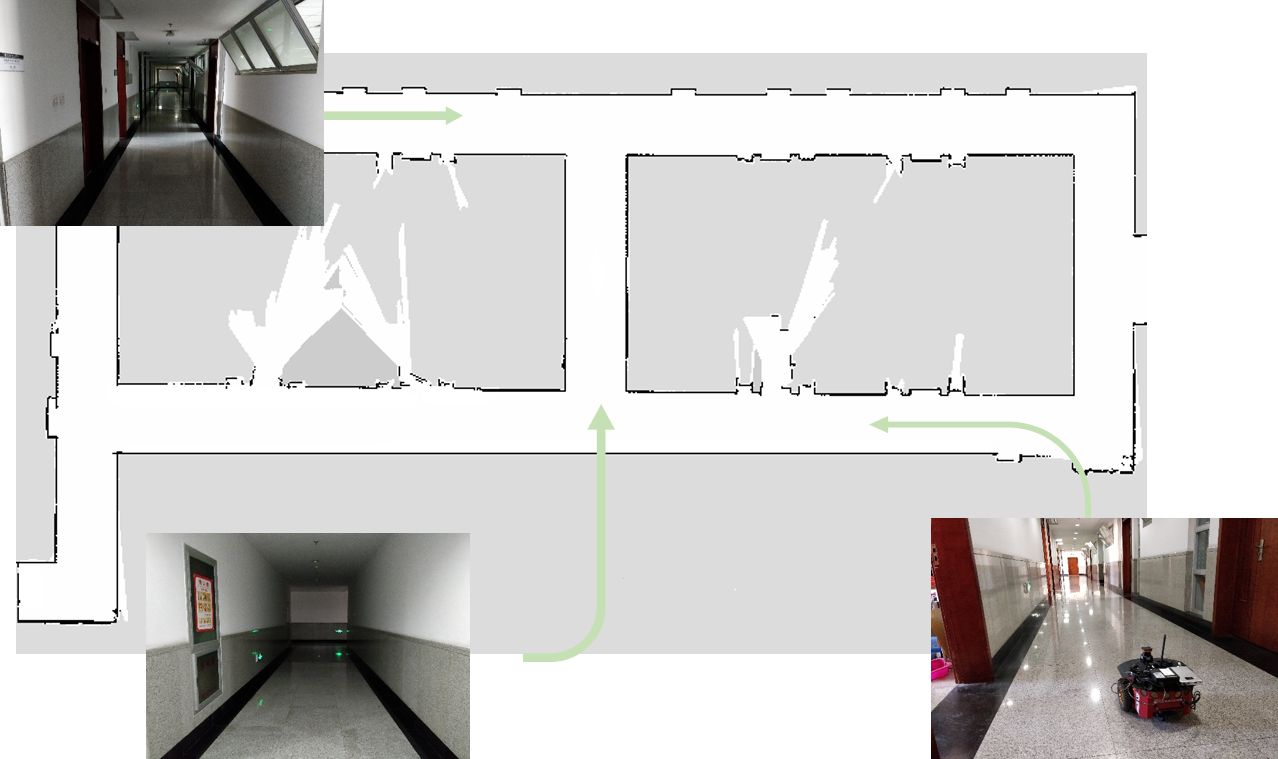
\includegraphics[width=0.45\textwidth]{map2.png}
	\caption{Priori map \uppercase\expandafter{\romannumeral2} of the real environment used to collect the data set.The white pixels represent the area without obstacles,the black pixels represent areas with obstacles and the gray pixels represent unknown area.}
	 \label{fig:map2}
\end{figure}

\subsection{Dataset and Training}

In order to obtain enough data for training, we gather 2D laser point clouds with poses in a real environment indoors with symmetrical similar structure as is show in Fag. \ref{fig:map1}. There is a d Pioneer 3-DX robot mounted with a Hokuyo UTM-30LX 2D laser scanner (shown in Fig. \ref{fig:robot}). The maximum linear and angular velocities of the robot are 0.6m/s and 1.0rad/s, respectively. The maximum measurement range of the laser scanner is 30.0m, and wide angle is 270. The ground truth positions $ [x, y, \theta] ^T$ and the range measurements are recorded at the speed of 3Hz. The environment used to collect the data sets is as shown in Fag. \ref{fig:map1}.

To validate that the convnet is regressing pose beyond that of the training examples we show the performance of the system in test dataset.The results shows that  our performance exceeds this we conclude that the convnet is successfully able to regress pose beyond training examples (shown in Fag.\ref{fig:point}).


\begin{figure}[H]
	\centering
	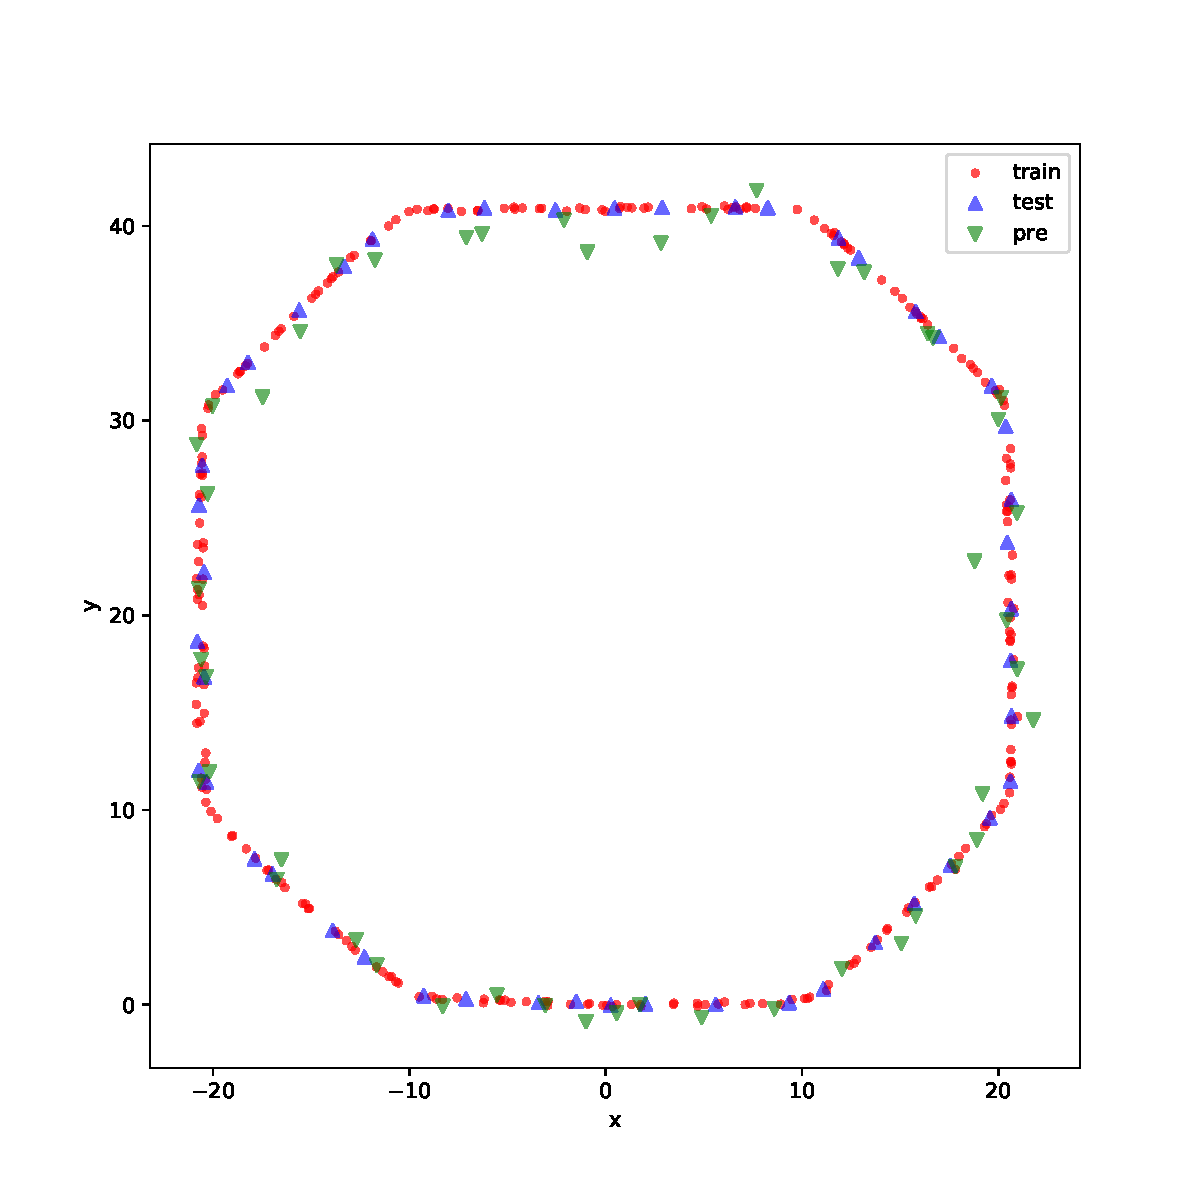
\includegraphics[width=0.4\textwidth]{point.pdf}
	\caption{Magnified view of a sequence of training (red) and testing (blue) data for scene \uppercase\expandafter{\romannumeral1}. We show the predicted robot pose in green for each testing frame. This shows our system can interpolate robot pose effectively in space between training frames.} \label{fig:point}
\end{figure}


\begin{figure}[H]
	\centering
	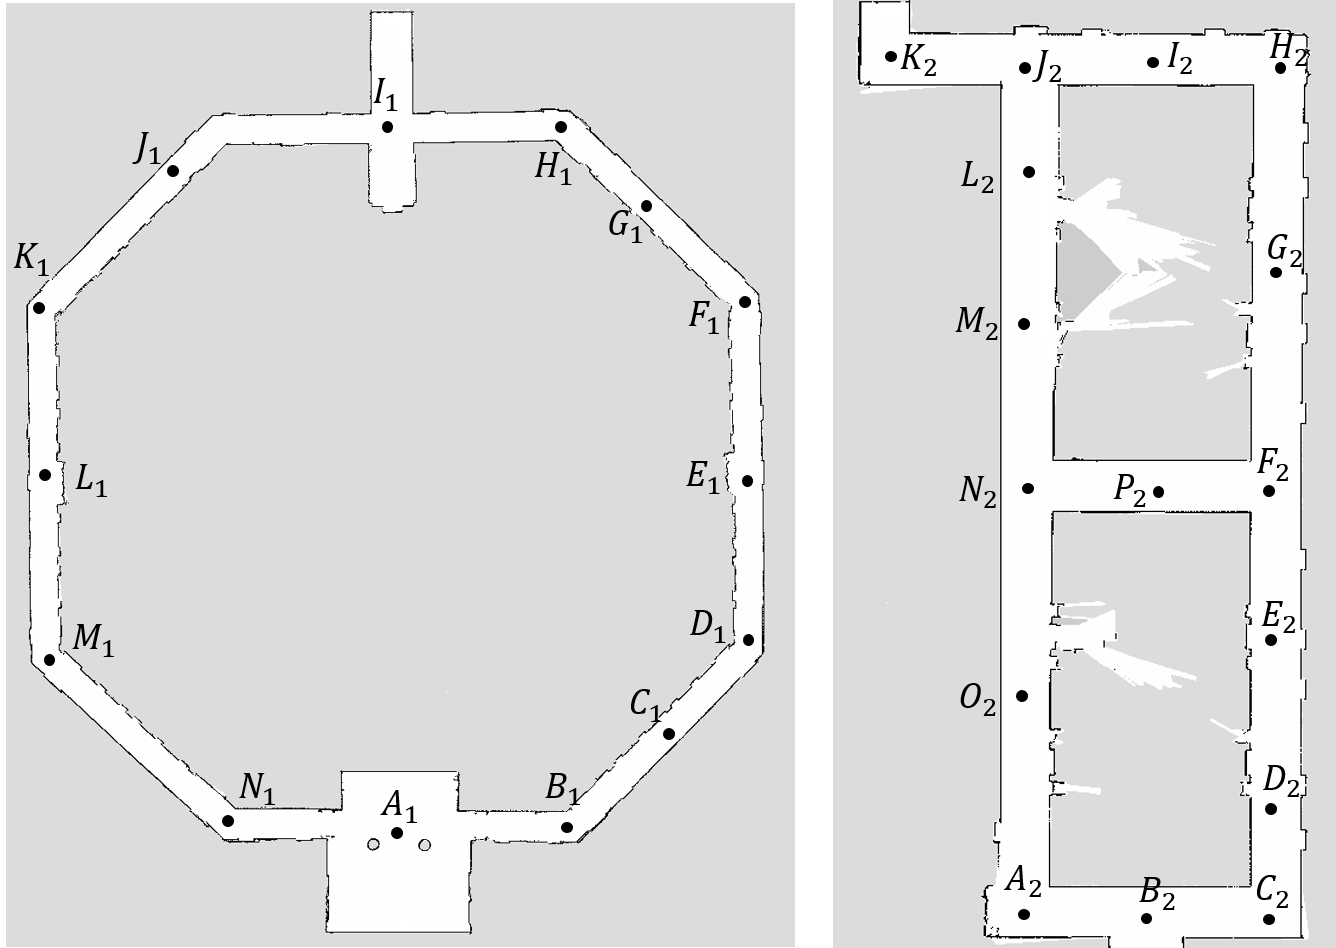
\includegraphics[width=0.4\textwidth]{testpoint1.png}
	\caption{ shows the  poses selected to test both particle filter algorithm and \textbf{Relocation-Net}.} \label{fig:testpoint1}
\end{figure}

\begin{table*}[]
	\centering
	\caption{ System performance in environment \uppercase\expandafter{\romannumeral1}}
	\begin{tabular}{c|c|c|c|c}
		\hline
		Site $A_1$-$N_1$               & Way of Testing & Testing Time Each Site & $A_1$-$N_1$ & Test Success Rate \\ \hline
		Particle Filter Algorithm  & Rotate in Situ & 10                     &         &  2/140                \\ \hline
		Relo-Net + Particle Filter & Rotate in Situ & 10                     &         &  139/140           \\ \hline
	\end{tabular}
	\label{tablemap1} 
%\end{table*}

%\begin{table*}[]
	\centering
	\begin{tabular}{c|c|c|c|c|c|c|c|c|c|c|c|c|c|c} 
		\hline
		& $A_1$  & $B_1$ & $C_1$ & $D_1$ &$ E_1 $ & $F_1$ & $G_1$ & $H_1$ &$ I_1$  & $J_1$ & $K_1$ & $L_1$  & $M_1$ & $N_1$ \\ \hline
		Particle Filter Algorithm  & 1/10 & 0   & 0   & 0   & 0    & 0   & 0   & 0   & 1/10 & 0   & 0   & 0    & 0   & 0   \\ \hline
		Relo-Net + Particle Filter & 1    & 1   & 1   & 1   & 9/10 & 1   & 1   & 1   & 1    & 1   & 1   & 9/10 & 1   & 1   \\ \hline
	\end{tabular}
\end{table*}

\begin{table*}[]
	\centering
	\caption{ System performance in environment \uppercase\expandafter{\romannumeral2}}
	\begin{tabular}{c|c|c|c|c}
		\hline
		Site $A_2$-$P_2$               & Way of Testing & Testing Time Each Site & $A_2$-$P_2$ & Test Success Rate \\ \hline
		Particle Filter Algorithm  & Rotate in Situ & 10                     &         &  6/160                \\ \hline
		Relo-Net + Particle Filter & Rotate in Situ & 10                     &         &  158/160           \\ \hline
	\end{tabular}
	\label{tablemap2} 
%\end{table*}

%\begin{table*}[]
	\centering
	\begin{tabular}{c|c|c|c|c|c|c|c|c|c|c|c|c|c|c|c|c}
		\hline
		& $A_2$  & $B_2$ & $C_2$ & $D_2$ &$ E_2 $ & $F_2$ & $G_2$ & $H_2$ &$ I_2$  & $J_2$ & $K_2$ & $L_2$  & $M_2$ & $N_2$ & $O_2$ & $P_2$ \\ \hline
		Particle Filter Algorithm  & 0   & 2/10 & 0   & 0   & 0   & 1/10 & 0    & 0   & 0   & 3/10 & 0   & 0   & 0    & 0   & 0   & 0   \\ \hline
		Relo-Net + Particle Filter & 1   & 1    & 1   & 1   & 1   & 1    & 9/10 & 1   & 1   & 1    & 1   & 1   & 9/10 & 1   & 1   & 1   \\ \hline
	\end{tabular}
\end{table*}


\begin{table*}[]
	\centering
	\caption{ Different forms of CNN Input in Scene \uppercase\expandafter{\romannumeral1}}
	\begin{tabular}{c|c|c|c|c|c|c}
		\hline
		The Input of CNN & Scene                                  & Mini Batch Number & Training Time & Training Frames & Testing Frames & Mean Accuracy on Test Set \\ \hline
		3-channel        & \uppercase\expandafter{\romannumeral1} & 6                 & 10h           & 4803            & 4180           & 5.543m                    \\ \hline
		6channel         & \uppercase\expandafter{\romannumeral1} & 6                 & 14h           & 4803            & 4180           & \textbf{1.920m}            \\ \hline
		12-channel       & \uppercase\expandafter{\romannumeral1} & 6                 & 22h           & 4803            & 4180           & 1.900m                   \\ \hline
		18-channel       & \uppercase\expandafter{\romannumeral1} & 6                 & 26h           & 4803            & 4180           & 1.912m                    \\ \hline
	\end{tabular}
	\label{tabchan1} 
\end{table*}


\begin{table*}[]
	\centering
	\caption{ Different forms of CNN Input in Scene \uppercase\expandafter{\romannumeral2}}
	\begin{tabular}{c|c|c|c|c|c|c}
		\hline
		The Input of CNN & Scene                                  & Mini Batch Number & Training Time & Training Frames & Testing Frames & Mean Accuracy on Test Set \\ \hline
		3-channel        & \uppercase\expandafter{\romannumeral2} & 6                 & 9h           & 4750            & 3500           & 4.540m                    \\ \hline
		6channel         & \uppercase\expandafter{\romannumeral2} & 6                 & 14h           & 4750            & 3500           & \textbf{1.87m}            \\ \hline
		12-channel       & \uppercase\expandafter{\romannumeral2} & 6                 & 22h           & 4750            & 3500          & 1.845m                     \\ \hline
		18-channel       & \uppercase\expandafter{\romannumeral2} & 6                 & 26h           & 4750           & 3500           & 1.834m                    \\ \hline
		\end{tabular}
		\label{tabchan2} 
	\end{table*}


\begin{figure}[H]
	\centering
	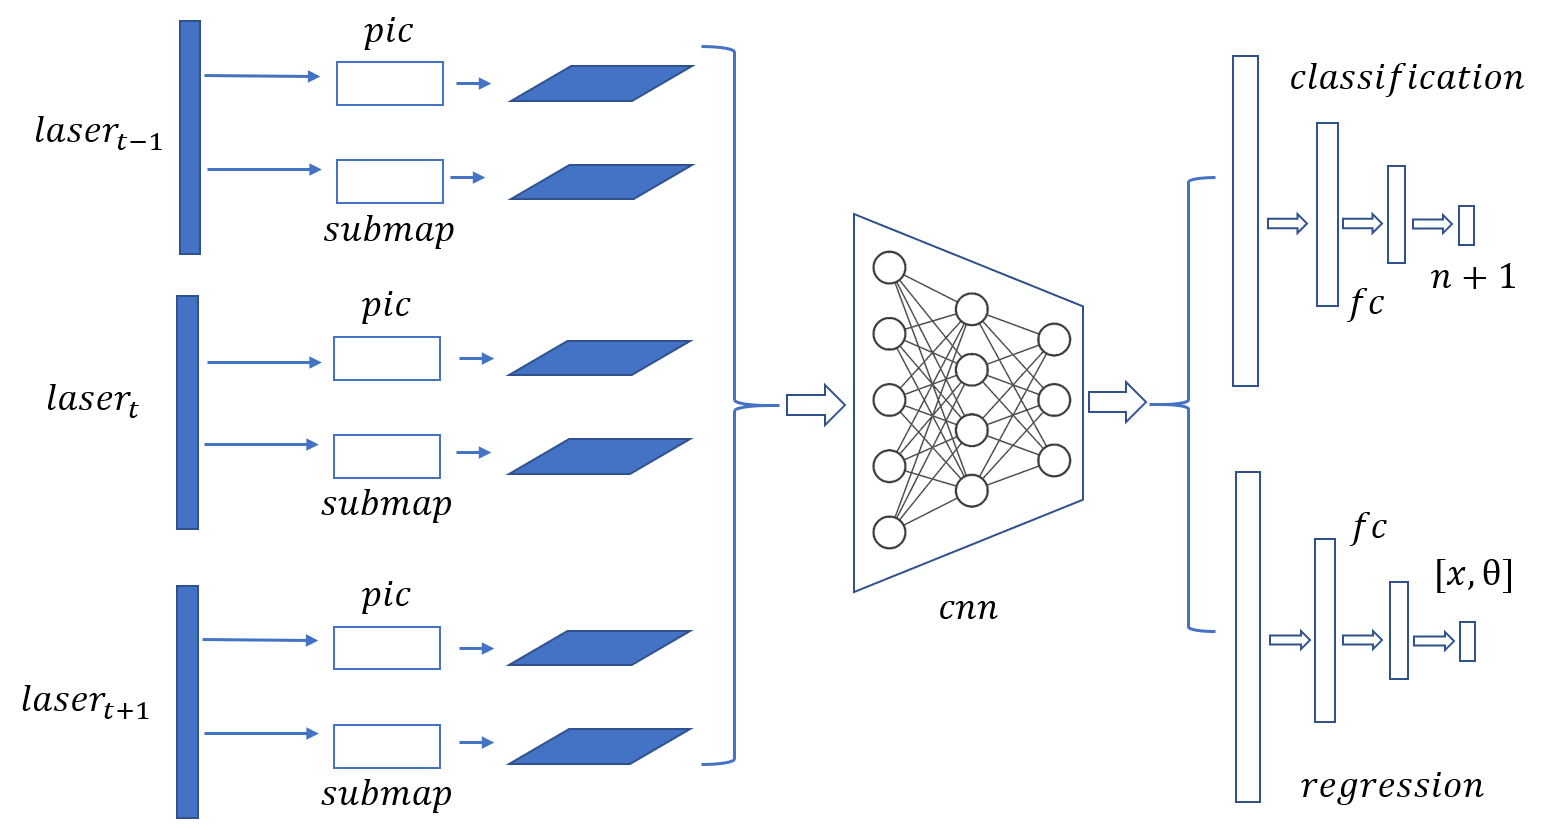
\includegraphics[width=0.5\textwidth]{net2.png}
	\caption{System overview of the Improved relocation algorithm for robot relocalization indoors. Part regression is used to predict robot pose. Part classification is used to distinguish the scene robot in.} 
	\label{fig:net2}
\end{figure}

\begin{figure}[H]
	\centering
	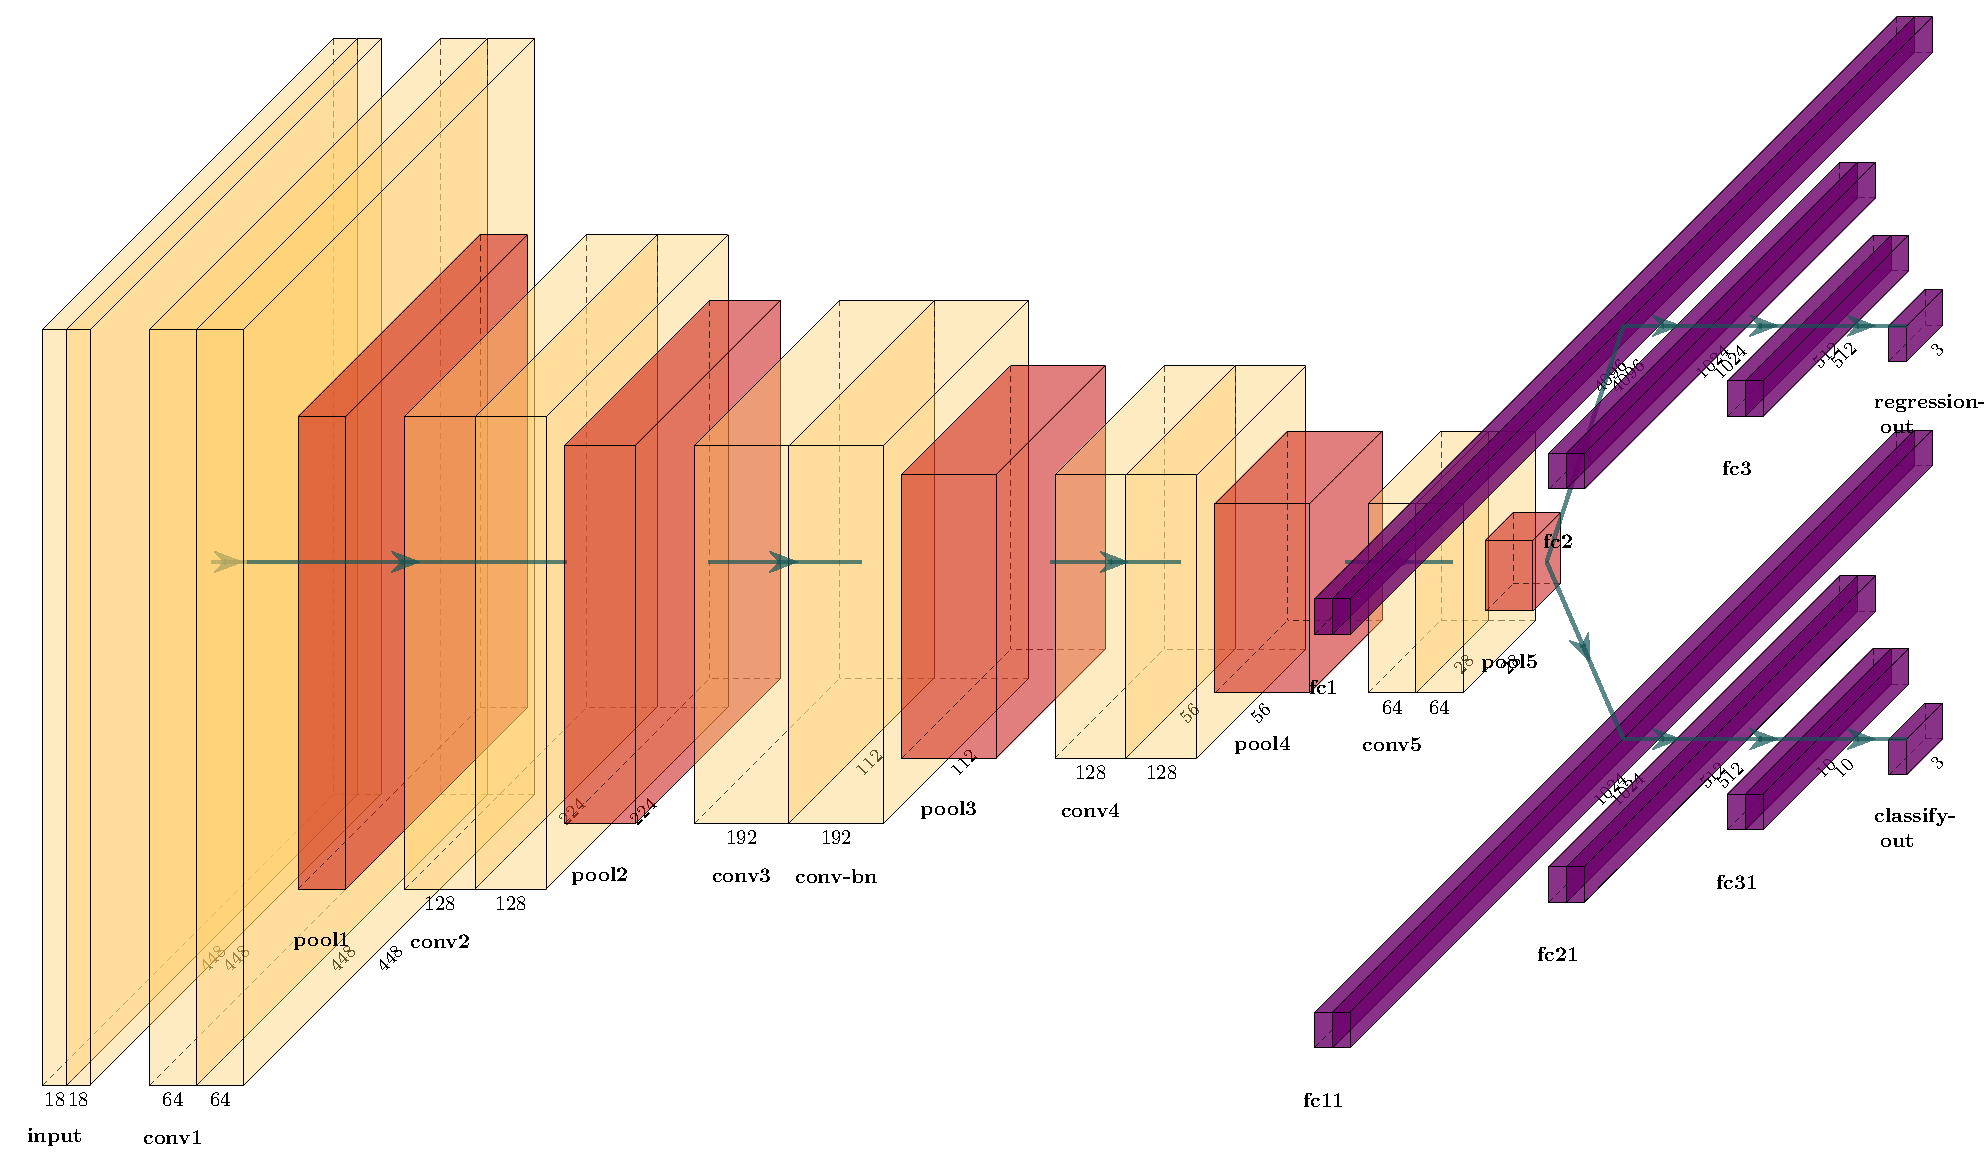
\includegraphics[width=0.5\textwidth]{fc.pdf}
	\caption{System overview of the Improved relocation algorithm for robot relocalization indoors. Part regression is used to predict robot pose. Part classification is used to distinguish the scene robot in.} 
	\label{fig:fc}
\end{figure}

\subsection{System Performance}

In order to prove the effectiveness of the our system, we conducted repeated experiments in the locations shown in Fag.\ref{fig:testpoint1}. We tested particle filter algorithm and our  particle filter algorithm optimized by our algorithm. 

As is shown in TABLE.\ref{tablemap1}, TABLE.\ref{tablemap2}, we tested effectiveness of the our system. We selected test sites in two real scenarios and conducted 10 tests in each location, and the test results were shown in the table. In the process of robot relocation, the traditional particle filter algorithm cannot solve the kidnapped robot problem in the similar structure environment, but our system can avoid the step of global particle distribution in the process of particle filter algorithm, so the kidnapped robot problem in the similar environment can be fundamentally solved.



\subsection{Different Forms of the Input}

In order to obtain a stable system and use the least computational resources, we used 3-channel, 6-channel, 12-channel and 18-channel images as the input of the neural network respectively, and compared their average measurement accuracy and computational resource consumption on the same test set(Shown in Table.\ref{tabchan1} and Table.\ref{tabchan2}).


\subsection{Multi-scene Mixed Training}

It is well known that indoor robot location relies on prior map. In order to verify that our system can not only  regress  robot posture, but also could identify the scene where the robot is. We  improved  our system so that it can classify scenarios. Fig.\ref{fig:net2} shows the improved network architecture,  part regression is used to predict robot pose and art classification is used to distinguish the scene robot in. We found that training individual networks to regress position and classify scene separately performed poorly compared to when they were trained simultaneously. We classified and annotated the same number of data sets in scenario 1 and scenario 2, and merged them into a new data set to serve as the input of the improved neural network.

We found that the improved neural network structure had no effect on the accuracy of posture regression, but it increased the training time by about 30 $\%$, and the classification accuracy reached 98.6$\%$.


\subsection{Real-Time Performance}

We test our system on a IPC(Industrial Personal Computer) (Intel Core TM Dual Core i7H-6500 and 6GB RAM) for the real-time performance. Our system doesn't need to run in real time, it just needs to predict the robot's position when the robot starts up. Our system only consumes 0.5s without the GPU.


\subsection{Discussion}


This paper proposes a method for indoor robot relocation based on convolutional neural networks. Firstly, a 2-D laser data preprocessing method is proposed to increase the position information in the input of neural network , and then the convolutional neural network model is designed to regress the robot pose. This method is based on the improvement of the traditional particle filtering algorithm. In the particle initialization step, the particles are distributed near the real position of the robot, thereby solving the "particle abduction problem" that occurs when the indoor robot restarts at any point. This paper also improves the neural network structure of the design, adding a scene classification module, so that the robot can identify the scene.

Since the subsequent particle filtering algorithm relies too much on the position predicted by the neural network, if the predicted position is wrong, the result of the robot positioning failure will occur.


\section{Conclusion and future work}

We present, to our knowledge, the first application of deep convolutional neural networks to  relocate robot pose indoors. We show that the kidnapped robot problem can be avoided during particle initialization. We showed that such networks preserve ample pose information in their feature vectors. Most importantly, we demonstrated that indoor robot repositioning can be achieved by relying only on two-dimensional laser sensors.

In future work, we will consider the issue of sensor fusion. We consider the use of fused data from odometers and two-dimensional lasers or fusion data of sonar and two-dimensional lasers as inputs to neural networks, which will increase the input characteristics of neural networks. It is obvious that a finite neural network has an upper bound on the physical area that it can learn to localize within, which we are going to  find this limit.

\appendices

%\section{Proof of the First Zonklar Equation}
%Appendix one text goes here.

%\section{}
%Appendix two text goes here.


% use section* for acknowledgment
%\section*{Acknowledgment}


%The authors would like to thank...

% Can use something like this to put references on a page
% by themselves when using endfloat and the captionsoff option.
%\ifCLASSOPTIONcaptionsoff
 % \newpage
%\fi


%\begin{thebibliography}{1}


%\end{thebibliography}


%\begin{IEEEbiography}{Michael Shell}
%Biography text here.
%\end{IEEEbiography}

% if you will not have a photo at all:
%\begin{IEEEbiographynophoto}{John Doe}
%Biography text here.
%\end{IEEEbiographynophoto}

% insert where needed to balance the two columns on the last page with
% biographies
%\newpage

%\begin{IEEEbiographynophoto}{Jane Doe}
%Biography text here.
%\end{IEEEbiographynophoto}

%\renewcommand\refname{Reference}
% that's all folks

\bibliography{wenxian}   %%% wenxian is here          !!!!!!!!!!!!!!!!!!!!!!
\end{document}



